\documentclass[a4paper, 12pt]{article}
%\documentclass[a4paper, 12pt]{skthesis}
\usepackage[english]{babel}
%\usepackage{lgrind}
\usepackage{cmap}
\usepackage[T2A]{fontenc}

\usepackage[utf8]{inputenc}
%Includes "References" in the table of contents
\usepackage[nottoc]{tocbibind}

\usepackage{cite}
\usepackage{amsmath,amssymb,amsfonts}
\usepackage{graphicx}
\usepackage{float}
\usepackage{textcomp}
\usepackage{xcolor}
\usepackage{amssymb}
\usepackage{hyperref}
\usepackage{subcaption}
\usepackage{dblfloatfix}
\usepackage{epstopdf}
\usepackage{diagbox}
\usepackage{csquotes}
\usepackage{adjustbox}
\usepackage{booktabs}
\usepackage{url}
%\usepackage{algorithm}
%\usepackage{algpseudocode}
%\usepackage{textgreek}
%\usepackage{bbding}
\usepackage{pifont}
\usepackage{wasysym}
\usepackage{amssymb}
\usepackage{color,colortbl}
\usepackage{calc}
\usepackage{stackengine}
\usepackage{array}
\usepackage{booktabs}
\usepackage{enumitem}
\usepackage{multirow}
\usepackage{makecell}
\usepackage{caption}
\usepackage{longtable}
\usepackage{lscape}
\usepackage{graphicx}

\usepackage{blindtext}
\usepackage{enumitem}

\usepackage{lipsum}

\title{thesis draft navigation. \\
Design of smartphone based SLAM algorithm for indoor crowd-source mapping.
}
\author{timur.chikichev }
\date{November 2020}

\begin{document}
	

%	% -*-latex-*-
% NOTE:
% These templates make an effort to conform to the Skoltech Thesis specifications,
% however the specifications can change.  We recommend that you verify the
% layout of your title page with your thesis advisor and the Education department 
% before printing your final copy.
\title{Indoor SLAM based on crowdsourced data with multiple smartphone sensors}

\author{Timur Chikichev}
% If you wish to list your previous degrees on the cover page, use the 
% previous degrees command:
%       \prevdegrees{MSc, University of Salzburg (2007)}
% You can use the \\ command to list multiple previous degrees
%       \prevdegrees{B.S., University of California (1978) \\
%                    S.M., Massachusetts Institute of Technology (1981)}
\department{Skoltech Center of Research, Entrepreneurship and Innovation}

\degree{Master Program in Space and Engineering Systems}

\degreemonth{November}
\degreeyear{2021}
\thesisdate{May 2021}

%% By default, the thesis will be copyrighted to MIT.  If you need to copyright
%% the thesis to yourself, just specify the `vi' documentclass option.  If for
%% some reason you want to exactly specify the copyright notice text, you can
%% use the \copyrightnoticetext command.  
%\copyrightnoticetext{\copyright \@author \@degreeyear}

% If there is more than one supervisor, use the \supervisor command
% once for each.
\supervisor{Edward Crawley}{Founding President, Professor}

% This is the department committee chairman, not the thesis committee
% chairman.  You should replace this with your Department's Committee
% Chairman.
%\chairman{Name}{Title}

% Make the titlepage based on the above information.  If you need
% something special and can't use the standard form, you can specify
% the exact text of the titlepage yourself.  Put it in a titlepage
% environment and leave blank lines where you want vertical space.
% The spaces will be adjusted to fill the entire page.  The dotted
% lines for the signatures are made with the \signature command.
\maketitle

% The abstractpage environment sets up everything on the page except
% the text itself.  The title and other header material are put at the
% top of the page, and the supervisors are listed at the bottom.  A
% new page is begun both before and after.  Of course, an abstract may
% be more than one page itself.  If you need more control over the
% format of the page, you can use the abstract environment, which puts
% the word "Abstract" at the beginning and single spaces its text.

%% You can either \input (*not* \include) your abstract file, or you can put
%% the text of the abstract directly between the \begin{abstractpage} and
%% \end{abstractpage} commands.

% First copy: start a new page, and save the page number.
\cleardoublepage
% Uncomment the next line if you do NOT want a page number on your
% abstract and acknowledgments pages.
% \pagestyle{empty}
\setcounter{savepage}{\thepage}
\begin{abstractpage}
\kant[1-2]
\end{abstractpage}


\clearpage
%\section*{Publications}
\subsection*{Main author}
\nobibliography*
\begin{enumerate}
    \item \bibentry{Skoltech2017}
\end{enumerate}

\subsection*{Co-author}
\begin{enumerate}
    \item \bibentry{Skoltech2017}
\end{enumerate}

\cleardoublepage

%\begin{dedication}
%Dedicated to my parents.
%\end{dedication}

\section*{Acknowledgments}

Let me thank to all my supporters.

Saian Protasov, Pavel Kopanev, Behnoosh Meskoob, Nikita Grunt - the team, we developed the idea of a current research. \\
Alexey Nikolaev, Maxim Ivanov, Alessandro Golkar - advisors of business and technology research related for this project. \\ 
Evgenia, Expomap CEO; Constantin, director of Metal expo - exhibitions organizers and experts, contributed in the business model statement of this project. \\
Research Advisor and Supervisor: Gonzalo Ferrer. 
Co-Advisor: Tatiana Podladchikova.

 % Your title pages, abstracts and acknowledgments
%	\tableofcontents
\newpage
\listoffigures
\newpage
\listoftables

 % Probably you don't need to change it%
%	%% This is an example first chapter.  You should put chapter/appendix that you
%% write into a separate file, and add a line \include{yourfilename} to
%% main.tex, where `yourfilename.tex' is the name of the chapter/appendix file.
%% You can process specific files by typing their names in at the 
%% \files=
%% prompt when you run the file main.tex through LaTeX.
\chapter{Introduction}

Micro-optimization is a technique to reduce the overall operation count of
floating point operations.  In a standard floating point unit, floating
point operations are fairly high level, such as ``multiply'' and ``add'';
in a micro floating point unit ($\mu$FPU), these have been broken down into
their constituent low-level floating point operations on the mantissas and
exponents of the floating point numbers.

Chapter two describes the architecture of the $\mu$FPU unit, and the
motivations for the design decisions made.

Chapter three describes the design of the compiler, as well as how the
optimizations discussed in section~\ref{ch1:opts} were implemented.

Chapter four describes the purpose of test code that was compiled, and which
statistics were gathered by running it through the simulator.  The purpose
is to measure what effect the micro-optimizations had, compared to
unoptimized code.  Possible future expansions to the project are also
discussed.

\section{Motivations for micro-optimization}

The idea of micro-optimization is motivated by the recent trends in computer
architecture towards low-level parallelism and small, pipelineable
instruction sets \cite{latexcompanion,einstein}.  By getting rid of more
complex instructions and concentrating on optimizing frequently used
instructions, substantial increases in performance were realized.

Another important motivation was the trend towards placing more of the
burden of performance on the compiler.  Many of the new architectures depend
on an intelligent, optimizing compiler in order to realize anywhere near
their peak performance
\cite{latexcompanion,einstein,knuthwebsite}.  In these cases, the
compiler not only is responsible for faithfully generating native code to
match the source language, but also must be aware of instruction latencies,
delayed branches, pipeline stages, and a multitude of other factors in order
to generate fast code \cite{latexcompanion}.

Taking these ideas one step further, it seems that the floating point
operations that are normally single, large instructions can be further broken
down into smaller, simpler, faster instructions, with more control in the
compiler and less in the hardware.  This is the idea behind a
micro-optimizing FPU; break the floating point instructions down into their
basic components and use a small, fast implementation, with a large part of
the burden of hardware allocation and optimization shifted towards
compile-time.

Along with the hardware speedups possible by using a $\mu$FPU, there are
also optimizations that the compiler can perform on the code that is
generated.  In a normal sequence of floating point operations, there are
many hidden redundancies that can be eliminated by allowing the compiler to
control the floating point operations down to their lowest level.  These
optimizations are described in detail in section~\ref{einstein}.

\section{Description of micro-optimization}\label{ch1:opts}

In order to perform a sequence of floating point operations, a normal FPU
performs many redundant internal shifts and normalizations in the process of
performing a sequence of operations.  However, if a compiler can
decompose the floating point operations it needs down to the lowest level,
it then can optimize away many of these redundant operations.  

If there is some additional hardware support specifically for
micro-optimization, there are additional optimizations that can be
performed.  This hardware support entails extra ``guard bits'' on the
standard floating point formats, to allow several unnormalized operations to
be performed in a row without the loss information\footnote{A description of
the floating point format used is shown in figures~\ref{exponent-format}
and~\ref{mantissa-format}.}.  A discussion of the mathematics behind
unnormalized arithmetic is in appendix~\ref{unnorm-math}.

The optimizations that the compiler can perform fall into several categories:

\subsection{Post Multiply Normalization}

When more than two multiplications are performed in a row, the intermediate
normalization of the results between multiplications can be eliminated.
This is because with each multiplication, the mantissa can become
denormalized by at most one bit.  If there are guard bits on the mantissas
to prevent bits from ``falling off'' the end during multiplications, the
normalization can be postponed until after a sequence of several
multiplies\footnote{Using unnormalized numbers for math is not a new idea; a
good example of it is the Control Data CDC 6600, designed by Seymour Cray.
\cite{knuthwebsite} The CDC 6600 had all of its instructions performing
unnormalized arithmetic, with a separate {\tt NORMALIZE} instruction.}.

% This is an example of how you would use tgrind to include an example
% of source code; it is commented out in this template since the code
% example file does not exist.  To use it, you need to remove the '%' on the
% beginning of the line, and insert your own information in the call.
%
%\tagrind[htbp]{code/pmn.s.tex}{Post Multiply Normalization}{opt:pmn}

As you can see, the intermediate results can be multiplied together, with no
need for intermediate normalizations due to the guard bit.  It is only at
the end of the operation that the normalization must be performed, in order
to get it into a format suitable for storing in memory\footnote{Note that
for purposed of clarity, the pipeline delays were considered to be 0, and
the branches were not delayed.}.

\subsection{Block Exponent}

In a unoptimized sequence of additions, the sequence of operations is as
follows for each pair of numbers ($m_1$,$e_1$) and ($m_2$,$e_2$).
\begin{enumerate}
  \item Compare $e_1$ and $e_2$.
  \item Shift the mantissa associated with the smaller exponent $|e_1-e_2|$
        places to the right.
  \item Add $m_1$ and $m_2$.
  \item Find the first one in the resulting mantissa.
  \item Shift the resulting mantissa so that normalized
  \item Adjust the exponent accordingly.
\end{enumerate}

Out of 6 steps, only one is the actual addition, and the rest are involved
in aligning the mantissas prior to the add, and then normalizing the result
afterward.  In the block exponent optimization, the largest mantissa is
found to start with, and all the mantissa's shifted before any additions
take place.  Once the mantissas have been shifted, the additions can take
place one after another\footnote{This requires that for n consecutive
additions, there are $\log_{2}n$ high guard bits to prevent overflow.  In
the $\mu$FPU, there are 3 guard bits, making up to 8 consecutive additions
possible.}.  An example of the Block Exponent optimization on the expression
X = A + B + C is given in figure~\ref{opt:be}.

% This is an example of how you would use tgrind to include an example
% of source code; it is commented out in this template since the code
% example file does not exist.  To use it, you need to remove the '%' on the
% beginning of the line, and insert your own information in the call.
%
%\tgrind[htbp]{code/be.s.tex}{Block Exponent}{opt:be}

\section{Integer optimizations}

As well as the floating point optimizations described above, there are
also integer optimizations that can be used in the $\mu$FPU.  In concert
with the floating point optimizations, these can provide a significant
speedup.  

\subsection{Conversion to fixed point}

Integer operations are much faster than floating point operations; if it is
possible to replace floating point operations with fixed point operations,
this would provide a significant increase in speed.

This conversion can either take place automatically or or based on a
specific request from the programmer.  To do this automatically, the
compiler must either be very smart, or play fast and loose with the accuracy
and precision of the programmer's variables.  To be ``smart'', the computer
must track the ranges of all the floating point variables through the
program, and then see if there are any potential candidates for conversion
to floating point.  This technique is discussed further in
section~\ref{range-tracking}, where it was implemented.

The other way to do this is to rely on specific hints from the programmer
that a certain value will only assume a specific range, and that only a
specific precision is desired.  This is somewhat more taxing on the
programmer, in that he has to know the ranges that his values will take at
declaration time (something normally abstracted away), but it does provide
the opportunity for fine-tuning already working code.

Potential applications of this would be simulation programs, where the
variable represents some physical quantity; the constraints of the physical
system may provide bounds on the range the variable can take.
\subsection{Small Constant Multiplications}

One other class of optimizations that can be done is to replace
multiplications by small integer constants into some combination of
additions and shifts.  Addition and shifting can be significantly faster
than multiplication.  This is done by using some combination of
\begin{eqnarray*}
a_i & = & a_j + a_k \\
a_i & = & 2a_j + a_k \\
a_i & = & 4a_j + a_k \\
a_i & = & 8a_j + a_k \\
a_i & = & a_j - a_k \\
a_i & = & a_j \ll m \mbox{shift}
\end{eqnarray*}
instead of the multiplication.  For example, to multiply $s$ by 10 and store
the result in $r$, you could use:
\begin{eqnarray*}
r & = & 4s + s\\
r & = & r + r
\end{eqnarray*}
Or by 59:
\begin{eqnarray*}
t & = & 2s + s \\
r & = & 2t + s \\
r & = & 8r + t
\end{eqnarray*}
Similar combinations can be found for almost all of the smaller
integers\footnote{This optimization is only an ``optimization'', of course,
when the amount of time spent on the shifts and adds is less than the time
that would be spent doing the multiplication.  Since the time costs of these
operations are known to the compiler in order for it to do scheduling, it is
easy for the compiler to determine when this optimization is worth using.}.
\cite{einstein}

\section{Other optimizations}

\subsection{Low-level parallelism}

The current trend is towards duplicating hardware at the lowest level to
provide parallelism\footnote{This can been seen in the i860; floating point
additions and multiplications can proceed at the same time, and the RISC
core be moving data in and out of the floating point registers and providing
flow control at the same time the floating point units are active. \cite{knuthwebsite}}

Conceptually, it is easy to take advantage to low-level parallelism in the
instruction stream by simply adding more functional units to the $\mu$FPU,
widening the instruction word to control them, and then scheduling as many
operations to take place at one time as possible.

However, simply adding more functional units can only be done so many times;
there is only a limited amount of parallelism directly available in the
instruction stream, and without it, much of the extra resources will go to
waste.  One process used to make more instructions potentially schedulable
at any given time is ``trace scheduling''.  This technique originated in the
Bulldog compiler for the original VLIW machine, the ELI-512.
\cite{latexcompanion,einstein}  In trace scheduling, code can be
scheduled through many basic blocks at one time, following a single
potential ``trace'' of program execution.  In this way, instructions that
{\em might\/} be executed depending on a conditional branch further down in
the instruction stream are scheduled, allowing an increase in the potential
parallelism.  To account for the cases where the expected branch wasn't
taken, correction code is inserted after the branches to undo the effects of
any prematurely executed instructions.

\subsection{Pipeline optimizations}

In addition to having operations going on in parallel across functional
units, it is also typical to have several operations in various stages of
completion in each unit.  This pipelining allows the throughput of the
functional units to be increased, with no increase in latency.

There are several ways pipelined operations can be optimized.  On the
hardware side, support can be added to allow data to be recirculated back
into the beginning of the pipeline from the end, saving a trip through the
registers.  On the software side, the compiler can utilize several tricks to
try to fill up as many of the pipeline delay slots as possible, as
seendescribed by Gibbons. \cite{knuthwebsite}


 

\section{Structure}

introduction
motivation
state of the art systems
system design and architecture

background, what is system, what features, how does it works
data processing
slam and graph minimization
factor graphs, distance function, graph matching
trajectory generation
walking model

map construction
observations to map (approximation, regression), map to observations (as a sensor)
(sensor model), propagation model, slam / sam

conditioning on magnetic field data
what graphs / figures can be plotted

\section{Background and problem statement}

The topic of the project is related to the problem of indoor navigation. The context of the problem states that no GPS data are available at hand, which makes the use of usual navigation services impossible.

Most existing systems of indoor navigation require special mapping stage. Novel indoor navigation systems utilize the data recorded from users. This is what is called the crowd-source approach.

For real-time indoor navigation, in conditions where is no initial data is available, we have to pass stages of localization and mapping, which can be done simultaneously in SLAM approach. We aim to combine both SLAM and crowd-source approach for the best performance of positioning system.

The innovation of this research is in ability to provide same navigation services with less information and in more natural way, which means also the reduced cost of the system overall.

\section{Objectives}
We perform this research to create an indoor positioning system with special features. The objective of this research is to develop all algorithms needed to obtain these features.

We define an approach for dealing with the dead reckoning system. We propose a mapping algorithm using ARcore visual odometry for training and all-time pedestrian dead reckoning and magnetic mapping for operation.

We aim to develop the system, working without complicated sensors or physical landmarks as beacons. This is only a research interest because the current SOTA PDR systems are only secondary to other approaches.

The problem we solve and the scope can be formulated as the following: design the algorithm of collection and processing the data for mapping indoor location for the indoor localization application. The algorithm should be solvable, by means that it always converge if sufficient data is given.


We can write the criteria for the positioning system we develop.

Criteria for the proposed system:
\begin{enumerate}
	\item no prior map is available: the system can work as SLAM system (real-time navigation with no prior map)
	\item no special hardware for operation except smartphones: positioning accuracy enough for operation (1-2m is the usual accuracy in this conditions)
	\item the system aggregate data from many sources (crowd-source) and improves the localization accuracy
\end{enumerate}


We formulate several hypotheses we evaluate during research:

Hypotheses:
The technology of magnetic field navigation can be implemented and fine-tuned for indoor crowd-source SLAM

The data from magnetic field and inertial sensors is enough for running SLAM

The crowd-source system satisfies the system optimality conditions and improve the accuracy

The hypothesis 2 was not proved in existing systems. For most system, additional prior knowledge is needed. This is more the scientific interest to prove this hypothesis.

Two other hypotheses are more the engineering questions. We have to compare performance and robustness of our algorithm and systems to other state of the art approaches. However for our problem statement, there is no much systems that have achieved any reasonable accuracy (1-2m). So we aim to achieve the accuracy that can be compared to other methods only.

\section{Introduction}

\subsection{Related work}

We review the field of human indoor localization. We focus on crowd-source mapping, or mapping with limited sensor model (limited to existing infrastructure in building space and to sensors in human smartphones).
In this field there are many approaches so solve the sub-problems or parts of given problem. 

We know paper GraphSLAM based Crowd sourcing framework for indoor Wi-Fi fingerprinting\cite{7809951}. The approach of GraphSLAM is promising. We want to utilize more available spatial information.

The most promising results in terms of cheap sensor spatial information are magnetic maps. For magnetic fingerprinting there are well developed approaches.

One of well-known papers in magnetic fingerprinting is \cite{Grand20123AxisMF}. The authors present an approach for magnetic field mapping, in terms of not fingerprints, but a full grid mapping procedure. As a result of this mapping procedure we obtain a full filed image that is easy to work with.
The problem with this approach that we have to collect full grid measurements, which is a time consuming procedure. We want to get magnetic field map without additional mapping procedure, this approach is called crowd-source mapping. We collect the data from a set of human travel trajectories. Then we merge them in single noised image (only analogy representation for better understanding), and apply optimization procedure. We require the resulting image be smooth, so the optimization constraints must be set to satisfy the image denoizing procedure. This is just our idea and assumption that is have to be proved in further research.
We see some similarities here with \cite{6827640}.

However they are highly dependent(?? prove statement) on the data collection procedure. This algorithms also are not intended for standalone usage in terms of sensors fusion. E.g. requires either special mapping procedures or additional hardware devices - beacons.

There are few papers on magnetic and inertial based navigation. However they were not implemented in SLAM frameworks such as \cite{7809951}. Some of frameworks are a part of commercial interest and are not open source.

The interesting map construction algorithm were proposed in \cite{6827640}. 

The full system consists of three subsystems, i.e. Dead Reckoning Subsystem (DRS), Map Construction Subsystem (MCS), and Localization and Navigation Subsystem (LNS). 

Our intuition gives that Dead Reckoning Subsystem performs sensor fusion and smoothing. The localization and navigation subsystem utilities the existing map and the output of smoothed sensors measurements.

The map construction process is an optimization problem with some constraints.

In \cite{6827640}, authors propose universal framework with no prior information of building map structure.
But for real situation, the map of the building is known.
We can define an indicator function similar to SLAM occupied cells mapping (????)
With indicator function defined, we may fit the graph of trajectories to the building inner structure graph - topological map.

The similar approach with map constraints correction and re-sampling was shown in \cite{articleXia}. The paper utilizes a   particle   filter that combines PDR and RSSI data.

\section{Methodology / theoretical framework}

Graph matching

Our case: formulate situation with no wifi available data in local area

(A specific case of this problem) The graph matching problem is the “maximum weighted bipartite matching”,

which is defined as a matching on a bipartite graph with maximum sum of the weights of selected edges.

This problem is also known as the “assignment problem”. We utilize factor Graphs for such assignment of new data.

Matching problem proposed:

We now describe the problem formulation by modelling two graphs: the ground truth graph (location based information - building map) and the data graph, constructed during the online training phase of system from the crowd-sourced data of users walking in the environment.

We do not obtain a radio map which is needed for RSS-based localization. Instead, we collect a data-set of magnetic field fingerprints, tagged with their relative physical coordinates to previous position. This relative coordinates (graph type trajectory with approximate information on edges lengths).

From the data of two graphs: location map and fingerprints collection, we perform matching procedure, using multiple available methods.

The first procedure to apply is accept-reject method: all points in restricted location are blocked (person can’t go through walls and etc.). Secondly, we perform loop closure and data association using common algorithms:

%graph similarity algorithms (correlation, ​)

probabilistic approach (hidden Markov models)

Similarity measures:

What data we obtain in the data graph: heading, relative position, magnetic field direction. For multiple locations in same domain there can be lots of point with same of similar magnetic field direction. Instead, between any two points, there can be enough magnetic field disturbances, which will create enough information for distinguishing data, and mapping only location related data.

We can measure the similarity only between long enough tracklets(parts of trajectory e.g. frames) / edges.

The signal similarity measure cab be just a cross-covariance

%Measurement model
%We use the available sensors / modules of the usual smartphones: WiFi, compass and accelerometer measurements obtained from inertial-magnetic unit, gyroscope and human step count module.

%Inertial model
%Steps count, adaptive step / stride lenght estimation - step count modules are available in several smartphones.

\subsection{System architecture}

MCS
MCS first partitions the trajectories into segments, and then clusters them into a cluster set C. For each cluster in C, with trajectory matching procedure, we construct the graph by connecting the crossing trajectories. We estimate the boundaries of the graph (trajectories closest to the walls), its width (adjust to corridor dimension) and location of each trajectory given the position of trajectory in graph and graph absolute position. We store the walls relative position to the processed graph in additional structure W.

From generated graph data, we extract / resample the representative trajectory, or field approximation. The representative trajectory set is denoted by R. This trajectory set has no relation to trajectories and input data, but only to the magnetic field in the given location. The output of MCS is the constructed digital map characterized by X, R , and W.

LNS
LNS performs particle-filter-based localization and routing-like navigation easily without any human intervention. The particle filter (PF) for localization utilizes the physical constraint that one cannot walk through the walls in estimating the posterior probability distribution of the user’s location.

\section{measurements model}

acceleration data from IMU \\
magnetic field orientation vector \\
RSSI


\section{Transition model definition}

We consider the process is Markovian.
Copied all from \cite{articleXia}:

With  the  development  of  microelectromechanical  systems(MEMS),  a  few  MEMS-based  sensors  have  been  built  and incorporated  into  smartphones:  accelerometers,  gyroscopes,magnetometers,  etc.  These  sensors  can  be  used  to  provide information  on  the  user’s  actions.  Pedestrian  dead  reckon-ing  (PDR)  [10]  is  a  relative  navigation  technique  that  uses these sensors.

we propose a PDR-based  indoor positioningmethod  that  integrates  RSSI  with  indoor  environment  mapconstraints by using particle filters.

PDR-based indoor positioning can be expressed by the following equations

\begin{equation}
X_k = \
\begin{bmatrix} 
x_{t-1} \\
y_{t-1} 
\end{bmatrix} = \
\begin{bmatrix} 
x_{t-1} &+ l_k \sin(\theta_t) \\
y_{t-1} &+ l_k \cos(\theta_t) 
\end{bmatrix} + \
\begin{bmatrix} 
\delta_{x} \\
\delta_{y} 
\end{bmatrix}
\end{equation}

The orientation  updates is independent from $X_k$ updates, depends on accelerometer and gyro, same model.

Step   Detection:Android   mobile   phones   have   two kinds  of  sensors  to  monitor  steps:  step  counters  and  step detectors [25]. 

Peak detection is used in this paper for step detection

nonlinear step length estimation model based on statistics proposed by Weinberg [27]

\begin{equation}
s = k \sqrt[4]{a_{z max} - a_{z min}}
\end{equation}

The Android system computes orientation angles by using the  device’s  geomagnetic  sensors  in  combination  with  its accelerometers   [25].   Using   these   two   hardware   sensors,the  system  provides  data  for  the  following  three  orientation angles

The  device is NOT  assumed to  be pointing in the heading direction. Need to apply additional space transformation.

\subsection{RSSI methode}

Usual path-loss model:

\begin{equation}
PL(d) = PL(d0) + 10 \alpha \log{d / d_0} + \omega = 
PL(d0) + 10 \alpha \log{d / d_0} + N(0, \sigma^2_{\omega})
\end{equation}

where $d$ represents the Euclidean distance between the anchor node  and  the  receiver,d0represents  a  specified  distance,PL(d)and PL(d0)represent the RSSI at $d$ and $d_0$, respectively(in  dBm),  and $\alpha$ represents the  path  loss  exponent, which  is closely related to the ambient environment; $\omega$ is a zero-mean Gaussian distribution variable with variance $\sigma^2_{\omega}$.

The inverse function: 
\begin{equation}
d_i = d_0 \cdot 10 \frac{PL(d_i) - PL(d_0)}{10\alpha}
\end{equation}

Landmark model:

\begin{align}
f_i(x, y) &= d_i - \sqrt{(x - x_i)^2 + (y - y_i)^2} \\
min(x, y) &= min \sum_{i=1}^{m}[f_i(x, y)]^2, m \ge 3.
\end{align}

In paper author transform this to linear system, 

\begin{align}
AZ & = b \\
A &= \begin{bmatrix} 
1 - 2 x_1 - 2 y_1 \\
... \\
1 - 2 x_m - 2 y_m
\end{bmatrix} \\
Z &= \begin{bmatrix} 
x^2 + y^2 \\
x \\
y
\end{bmatrix} \\
b &= \begin{bmatrix} 
d_1^2 - x_1^2 - y_2^2\\
...\\
...
\end{bmatrix}
\end{align}

We have to check it

Good alternative was proposed in \cite{} to bound region by min and max RSSI according to its variance - linear system.

\subsection{Processing}

Update step, prediction, correction
State Estimation


Resample:In  this  step,  importance  resampling  [20]  isused to obtain a new particle set

some papers prove importance resampling can't be applied for this task because pf noise.
% observation equation:

% \section{Crasy Idea}

% There is some similarity in video compressing process

% We strore gradients of changing signal measurements, we apply searching procedure to have a smooth measurements.

% We have a convex magnetic field and a trajectory, 
% the task is to find similar trajectrory with highest correlation to measurements.

% Regression, approximation, pattern matching, Convolutions.

% Gradients, blockmatching

% Different approaches in papers, play on a toy model.


\subsection{RSSI Graph SLAM}

Definition taken from \cite{7809951}.

Trajectory Modelling with GraphSLAM\cite{SLAM_using_Gaussian_process_latent_variable_models}   is   a   classical   framework   for SLAM optimization.

GraphSLAM  extends  the  traditional  SLAM  framework  by considering  the  poses  in  a  trajectory  as  nodes  and  raw  measurements between poses and landmarks as edges in a graph.Note that each edge is attached with a probability distribution over  the  relative  positions  of  its  two  vertexes  since  inherent noise in sensors need to be considered. In 2-D case, a pose $x_t$ consists of a 2-D coordinates $(x_1,t,x_2,t)$ and an yaw angle $\theta_t$.

\begin{equation}
e_{i j}(x_i, x_j) = z_{i j} - \hat z_{i j} (x_i,x_j)
\end{equation}

The item $\omega_{i j}$ in the equation is the information matrix representing Gaussian noise in sensor measurement.The GraphSLAM problem is now reduced to a constrained least  square  problem  and  it  can  be  solved  by  some  standard optimization techniques, like Gaussian-Newton or Levenberg-Marquardt algorithms, as proposed in [16]. Either of the two methods is based on local iterative linearization: 
%x′=  ̆x+ ∆x

Then,  the  goal  of  GraphSLAM  is  to  find  an  configuration of  poses $x^{*}$ that  minimizes  the  squared  error F(x) of  all observations given a set of constraint edges C:

\begin{align}
F(X) =\sum_{(i,j)\in C} e_{i j}^T Ω_{ i j} e_{i j} \\
x^{*} = argmin_x F(x)
\end{align}


\section{factor graphs, distance function, graph matching}

%We need to define a distance function for further graph matching.
We define a distance function as a space measure/metric to construct a formal space as the Cartesian product of spaces.
We construct it in a way of traditional Borel set definition.

For any collection $E_{1..i}$ of a countable (possibly finite) number of pairwise disjoint, measurable sets, let $E$ denote their union. 
The measure $\mu$ for the iteration of the whole collection must satisfy:

\begin{equation*}
	\mu(E) = \sum_i \mu(E_i)
\end{equation*}

If we given the space of observations $(z, \rho_z)$ and the space of states $(x, \rho_x)$. And let $(z, \rho_z)$,   $(x, \rho_x)$ be two metric spaces.

We may define a composition distance function with the Cartesian product of given spaces:

\begin{equation}
	\rho_{x, z} (X_1, X_2) = c_1\rho_x (x_1, x_2) + c_2\rho_z (z_1, z_2)
\end{equation}

The traditional restriction is for the positive weights.

We plan use distances as the likelihood function, so here we do not really care about distances itself on a large scale, only as the similarity measure.

The $\rho_x$ is the traditional L2 distance, plus added angle delta function.
We refer to example from Lavalle book, $SO(2)$ Metric by Comparing Angles:

\begin{equation}
\rho(\theta_1, \theta_2) = \min\{|\theta_1 - \theta_2|, 2\pi - |\theta_1 - \theta_2|\}
\end{equation}

Or better in the continuous form as the inverse cosine of the complex number representation of angles $a + b i$:

\begin{equation}
\rho(\theta_1, \theta_2) =  \rho(a_1, b_1, a_2, b_2) = \cos^{-1}\{a_1 a_2 + b_1 b_2\}
\end{equation}
for two points $(a_1 , b_1 )$ and $(a_2 , b_2 )$

The alternative here is using the SE3 metric or quaternion based representation, but we don't consider them here for simplicity.

\subsection{SAM for magnetic localization problem}

\begin{align}
	P(X, M, Z, U) &= p(x_0)\prod_{i=1}^{M}p(x_i|x_{i-1}, \mu_i)\cdot \prod^{k}p(z_k|x_{i_k}) \\
	p(z_k|x_{i_k}) &= \log(z_k - h(x_{i_k}))
\end{align}

Objective: maximize the joint probability using graph theory and linear Algebra.

SAM problem is represented as a factor graph - bipartite graph with weighted nodes and edges.

\begin{align}
\theta &= \{X, M\}, \\
p(\theta) &= \prod \phi_i(\theta_i) \cdot \prod \xi_{ij}(\theta_i \theta_j) \\
\phi_0(x_0) &\propto p(x_0) \\
\phi_{i-1, i}(x_{i-1}, x_i) &\propto p(x_i|x_{i-1}, u_i) \\
\xi_{ij}(\theta_i \theta_j) &\propto p(z_k|x_{i_k}, M(x_{i_k})) 
\end{align}

Transition model
\begin{align}
p(x_i|x_{i-1}, u_i) &= N(x_i; g_i(x_{i-1}, u_i), \Sigma_{u_i})
\end{align}

The covariance matrix $\Sigma_{u_i}$ is constant here.

The function g() is defined by the propagation model. We have the traditional pedestrian dead reckoning problem statement. 
The inertial motion model is the following:



%Smoothing: optimization of the chain trajectory

Observation model
\begin{align}
p(z_k|x_{i_k}) &= N(z_k; h_k(x_{i_k}, m_{j_k}), \Sigma_{k}) \\
m_{j_k} &= M(x_{j_k})
\end{align}

\subsection{Clustering application for mapping}

The optimization task: global minimization, matrix reduce, ....

States are only locally dependent, thus the task can be approximately solved for local clusters. The single task can be parallelized and all minimization problems can be formulated and solved independently for sub-locations. 

We approximate the space, so we have to split a continuous space in a decent manner. The good way would be to use a constant area discrepancy trick as in regular random sampling methods. In Lavalle book the are a decent examples, but for simplicity we stay with a regular grid and RBF functions.

The grid and a measure function together define a cluster shape and specifics. We can use rbf or either an ellipse function (sum of distances to two points).

For each points in coordinates x-y of state space, we assign cluster c(x, y, m)

Clusters are an additional variables in state, linkages in lookup tables.

We are not restricted to lattices, because we allow clusters to overlap a bit. Thus the optimization problem will be solved twice or more time for overlapping vertices or states, which will guarantee smoothness in resultant solution.


\section{Experiments}

\subsection{Pose estimation and IMU Modelling}

\begin{figure}
	\centering
	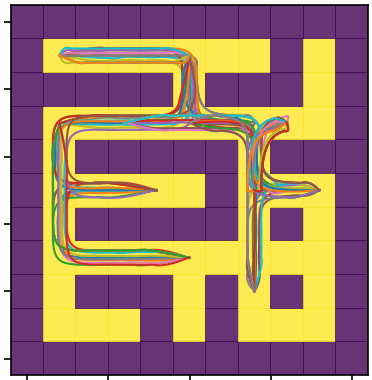
\includegraphics[width=0.4\linewidth]{images/routes2}
	\caption{Random trajectories on a generated building map.}
	\label{fig:routes1}
\end{figure}

We generate the series of data using maze generation algorithm. On a fixed map of corridors we generate routes and trajectories, then we add noise to simulate the walking human.

\begin{figure}
	\centering
	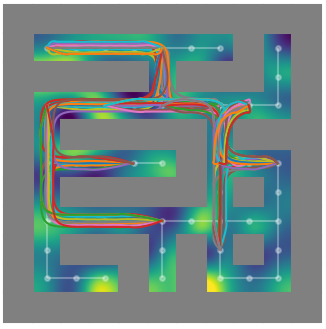
\includegraphics[width=0.7\linewidth]{images/routes3}
	\caption{The background simulates continuous random field we want to reconstruct}
	\label{fig:routes3}
\end{figure}


We simulated the walking model of the pedestrian using particle filter.

Current implementation is fully functional and flexible,
we run experiments on localization and navigation using this code.


\begin{figure}
	\centering
	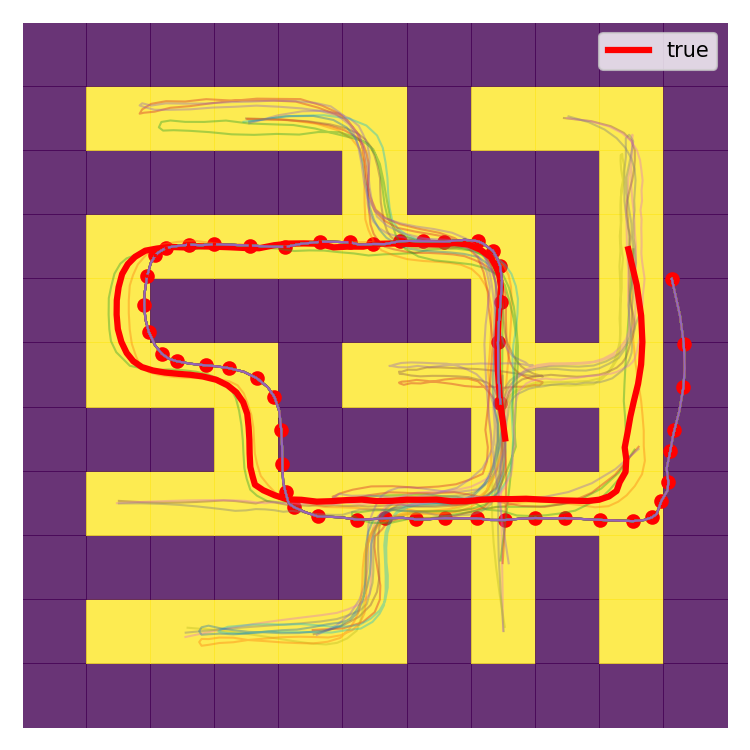
\includegraphics[width=0.7\linewidth]{images/Figure_dvwaerv1}
	\caption{Particle filter run}
	\label{fig:pf}
\end{figure}

On figure \ref{fig:pf} shown the true and simulated trajectories.
We have to add conditioning on observations, but this is a smalll minor update we will do later.

\begin{figure}
	\centering
	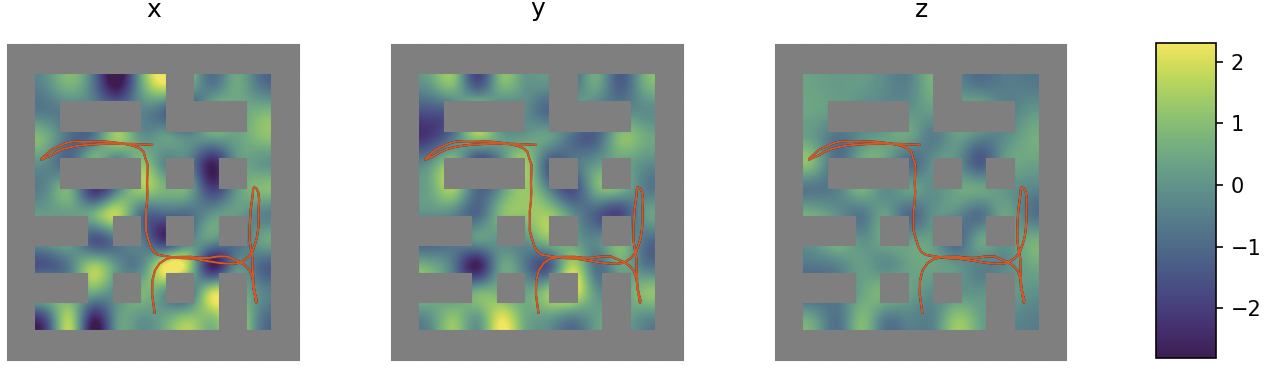
\includegraphics[width=0.99\linewidth]{images/Figure_1erhawrhser}
	\caption{Sensor model}
	\label{fig:Sensor_model}
\end{figure}

On figure \ref{fig:Sensor_model}, the sensor model is being shown.
We select 3 observations from 3 surfaces for each pose. All observations are later reconstructed to surface and then compared to true field data.

Once we have working filtering procedure, we have a tool for data mapping. The localization can be performed using same tool, but using the known reconstructed data.

\subsection{Data processing}

First we focus on a key part of a given research. The main part of this paper requires the transformation of observation to the solid continuous map.

After we highlighted the map structure and features, we can say that we need to reconstruct the magnetic field.

A magnetic field is continuous potential field with certain known features. Each point has its own field direction and magnitude.
We can encode the field as a number of three dimensional vectors or as 3 images, representing the field magnitude in each axis direction.

First we model the field construction and reconstruction. 

\subsubsection{image approximation}

We generate a surface from array with random noise values as a mesh and apply interpolation and smoothing.
On the random surface we sample a series of points. The problem is to accurately reconstruct the initial surface from samples.

There are  several possible solutions for such problem. The most promising and accurate seems kernel training as in Kernel Ridge Regression or other similar methods. From the other side, there are other more straightforward solutions.

Solution 1: interpolation. Solution is not accurate and not feasible because resulting surface is very noisy. We need a solution to deal with many observations and noisy data.

The promising solution was shown in repository of \cite{Surface_approximation_GP}. We aim to solve the problem in similar problem statement with more traditional methods.




\begin{figure}
	\centering
	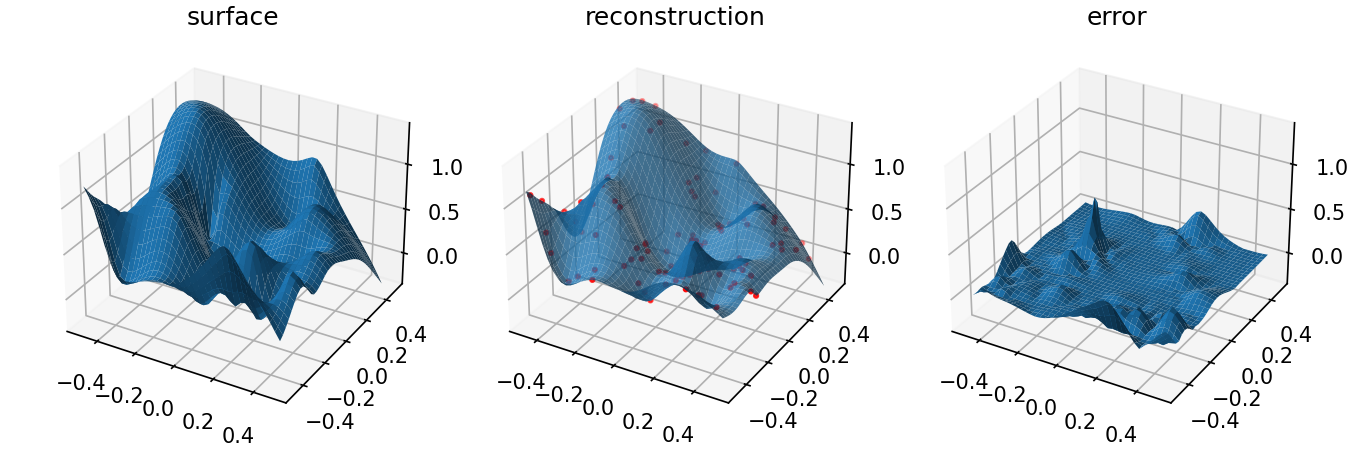
\includegraphics[width=1.0\linewidth]{images/rbfinterp3d}
	\caption{}
	\label{fig:rbfinterp3d}
\end{figure}

We perform the noisy surface approximation using RBF function from the scipy package.

On the figure \ref{rbfinterp3d}, the right plot represents the distance between initial and approximated surfaces.


\section{Work progress}

From the list of planned objectives, the uncompleted are the following:

Estimation of localization model’s performance in code simulation. \\
Smartphone implementation for sensing data collection. \\
Estimation of localization accuracy in real experiments. \\

We have to complete small number of experiments for algorithm accuracy estimation. 
Currently, we almost completed the work on localization on magnetic field data using the particle filter. The similar papers are \cite{Grand20123AxisMF, 7809951}.

%	\include{chapters/chapter3} 
%	\appendix
%	\chapter{Tables}


\clearpage
\newpage

%	\chapter{Figures}

\vspace*{-3in}

\begin{figure}
\vspace{2.4in}
\caption{Armadillo slaying lawyer.}
\label{arm:fig1}
\end{figure}
\clearpage
\newpage

\begin{figure}
\vspace{2.4in}
\caption{Armadillo eradicating national debt.}
\label{arm:fig2}
\end{figure}
\clearpage
\newpage

%	\bibliographystyle{plain}
\bibliography{main.bib}


We use the approach of surface approximation from \cite{Surface_approximation_GP}.


We need to complete motivation part, write all supporting text and equations for the models we use. 
This is absolutely possible task, because all derivations are already written in paper and implemented in code. 

The timeline of future actions to complete the thesis is defined.
In 3 more days, the graphics part and equations will be ready for thesis submission. Additional few days are needed to complile the roadmap and tecnological research as a motivational part of the thesis - e.g. preliminary research. 

Current presenation is available at \url{https://docs.google.com/presentation/d/1okQ8xhp4loKDlqegFuVSBieAd4HiGIXiI-SPlva9Efs/edit?usp=sharing}


The technology roadmap presentation \url{https://docs.google.com/presentation/d/17Y4y7kEfnQPwoDM8SHt8FAUGgpr_LoDErFYHAzCHLqE/edit?usp=sharing}. This data will be added to current document.

The latest technology roadmap paper on magnetic localization is available at \url{https://www.overleaf.com/read/fdjmmbbtwnkn}.  

The roadmap covers patent research, literature research and problem statement for the current thesis. The localization systems architecture is also highlighted.


Currently the is no problems in completing the thesis in remaining time. Sure, active work on text refactoring is required. This work will be done before external reviewer submission.

\subsection{Results readiness estimation}
The work completion percentage in my opinion is $75\%$.

All the data and code is submitted to github \url{https://github.com/notenoughsun/ms-thesis}.

The most work is currently contained at graph simulation, \url{https://github.com/notenoughsun/ms-thesis/tree/main/code/graph_gen}. Figures and derivations are also available there.

This paper is not yet compiled for submission. Most parts of research are not added to this document but will be added in few days.


\bibliographystyle{unsrt}
\bibliography{bib}

\end{document}
